%%
%% prog-folien
%%
%% Slides for my Java programming tutorial using LaTeX beamer.
%%
%% Copyright (c) 2015-2016 YouniS Bensalah <younis.bensalah@riseup.net>
%%
%% This work is released to the public domain.
%% For the full copyright and license information, please view the LICENSE file.
%%

%% LaTeX-Beamer template for KIT design
%% by Erik Burger, Christian Hammer
%% title picture by Klaus Krogmann
%%
%% version 2.1
%%
%% mostly compatible to KIT corporate design v2.0
%% http://intranet.kit.edu/gestaltungsrichtlinien.php
%%
%% Problems, bugs and comments to
%% burger@kit.edu

\documentclass[18pt]{beamer}

%% SLIDE FORMAT

% use 'beamerthemekit' for standard 4:3 ratio
% for widescreen slides (16:9), use 'beamerthemekitwide'

\usepackage{templates/beamerthemekit}
% \usepackage{templates/beamerthemekitwide}

\usepackage[utf8]{inputenc}
\usepackage{hyperref}
\usepackage{listings}
%\usepackage{xcolor}
%\usepackage{colortbl}
%\usepackage{array}
%\usepackage{tikz}
%\usetikzlibrary{calc,shapes.multipart,chains,arrows}

%\definecolor{lime}{HTML}{8FFF53}

\newcommand{\quotes}[1]{``#1''}

%% TITLE PICTURE

% if a custom picture is to be used on the title page, copy it into the 'logos'
% directory, in the line below, replace 'mypicture' with the
% filename (without extension) and uncomment the following line
% (picture proportions: 63 : 20 for standard, 169 : 40 for wide
% *.eps format if you use latex+dvips+ps2pdf,
% *.jpg/*.png/*.pdf if you use pdflatex)

\titleimage{greendrop}

%% TITLE LOGO

% for a custom logo on the front page, copy your file into the 'logos'
% directory, insert the filename in the line below and uncomment it

%\titlelogo{mylogo}

% (*.eps format if you use latex+dvips+ps2pdf,
% *.jpg/*.png/*.pdf if you use pdflatex)

%% TikZ INTEGRATION

% use these packages for PCM symbols and UML classes
% \usepackage{templates/tikzkit}
% \usepackage{templates/tikzuml}

% the presentation starts here

\title[Vererbung und Polymorphismus]{Programmieren:\\ Vererbung und Polymorphismus}
\subtitle{Tutorium 30}
\author{YouniS Bensalah}
\date{December 4, 2015}

\institute{Chair for Software Design and Quality}

% Bibliography

\usepackage[citestyle=authoryear,bibstyle=numeric,hyperref,backend=biber]{biblatex}
\addbibresource{templates/example.bib}
\bibhang1em

\begin{document}

% change the following line to "ngerman" for German style date and logos
\selectlanguage{english}

%title page
\begin{frame}
\titlepage
\end{frame}

%table of contents
\begin{frame}{Heute}
\tableofcontents
\end{frame}

\section{Vererbung}

\subsection{Unter- und Oberklassen}

\begin{frame}{Vererbung}
    \begin{itemize}
        \item \textbf{Vererbung} (\textit{inheritance}) erlaubt es, neue Klassen aus bestehenden aufzubauen.
        \item Dabei übernimmt (\textit{erbt}) die neue sog. \textbf{Unterklasse} alle Methoden und Attribute der \textbf{Oberklasse}.
        \begin{itemize}
            \item Die Unterklasse (\textit{subclass}) ist eine \textbf{Spezialisierung} der Oberklasse.
            \item Die Oberklasse (\textit{superclass}) ist eine \textbf{Generalisierung} der Unterklasse.
        \end{itemize}

    \end{itemize}
\end{frame}

\begin{frame}{is-a}
    Vererbung modelliert eine \alert{\quotes{is-a}}-Beziehung.
    \vspace{.2in}
    \begin{itemize}
        \item \texttt{Car} \alert{is a} \texttt{Vehicle}
        \item \texttt{Bird} \alert{is a} \texttt{Animal}
        \item \texttt{Manager} \alert{is a} \texttt{Employee}
        \item \texttt{Animal} \alert{is a} \texttt{LivingOrganism}
    \end{itemize}
\end{frame}


\begin{frame}[fragile]{Beispiel}
    \begin{columns}[c]
        \column{.5\textwidth}
            \begin{exampleblock}{}
                \begin{lstlisting}[language=Java,basicstyle=\scriptsize]
public class Dog {

    private String name;

    public void sayName() {
        System.out.println(this.name);
    }

    public void fetchStick() { ... }

}
                \end{lstlisting}

            \end{exampleblock}
        \column{.5\textwidth}
            \begin{exampleblock}{}
                \begin{lstlisting}[language=Java,basicstyle=\scriptsize]
public class Cat {

    private String name;

    public void sayName() {
        System.out.println(this.name);
    }

    public void sleep() { ... }

}
                \end{lstlisting}
            \end{exampleblock}
    \end{columns}

    \pause

    \begin{itemize}
        \item Redundanter Code: beide Klassen haben ein \texttt{name} Attribut und eine \texttt{sayName()} Methode !
        \item Zum Glück gibt es \textbf{Vererbung} in Java\dots
    \end{itemize}
\end{frame}

\begin{frame}[fragile]{Vererbung in Java: extends}
    \begin{itemize}
        \item Syntax:\\
\begin{lstlisting}[language=Java]
class A extends B { ... }
\end{lstlisting}
        \item Klasse \texttt{A} erweitert Klasse \texttt{B}
        \begin{itemize}
            \item \texttt{A} ist die Unterklasse (\textit{subclass})
            \item \texttt{B} ist die Oberklasse (\textit{superclass})
        \end{itemize}


    \end{itemize}
\end{frame}

\begin{frame}[fragile]{Beispiel (diesmal mit Vererbung)}
    \begin{columns}[c]
        \column{.5\textwidth}
            \begin{exampleblock}{}
                \begin{lstlisting}[language=Java,basicstyle=\scriptsize]
public class Dog extends Pet {

    public void fetchStick() { ... }

}

public class Cat extends Pet {

    public void sleep() { ... }

}
                \end{lstlisting}
            \end{exampleblock}
        \column{.5\textwidth}
            \begin{exampleblock}{}
                \begin{lstlisting}[language=Java,basicstyle=\scriptsize]
public class Pet {

    private String name;

    public void sayName() {
        System.out.println(this.name);
    }

}
                \end{lstlisting}
            \end{exampleblock}
    \end{columns}

    \begin{itemize}
        \item A \texttt{Dog} \textbf{is a} \texttt{Pet}
        \item A \texttt{Cat} \textbf{is a} \texttt{Pet}
    \end{itemize}
\end{frame}

\begin{frame}{Vererbung}
    Was genau wird eigentlich vererbt ?
    \vspace{.2in}
    \begin{itemize}
        \item Attribute
        \item Methoden
        \item Geschachtelte Klassen (\textit{nested classes})
    \end{itemize}
    \vspace{.2in}
    Aber\dots
    \begin{itemize}
        \item \alert{Konstruktoren werden \textit{nicht} vererbt !}
    \end{itemize}
\end{frame}

\begin{frame}[fragile]{Vererbung und Konstruktoren}
    \begin{exampleblock}{}
        \begin{lstlisting}[language=Java,basicstyle=\scriptsize]
public class Pet {

    private String name;

    public Pet(String name) {
        this.name = name;
    }

}

public class Cat extends Pet {

    public void sleep() { ... }

}
        \end{lstlisting}

    \end{exampleblock}
\end{frame}

\begin{frame}[fragile]{Vererbung und Konstruktoren}
    \begin{exampleblock}{}
        \begin{lstlisting}[language=Java,basicstyle=\scriptsize]
Cat c = new Cat("Garfield");
        \end{lstlisting}

    \end{exampleblock}

    \begin{itemize}
        \item Das geht schief !
        \item Die Klasse \texttt{Cat} kennt keinen Konstruktor mit der Signatur: \texttt{Cat(String name)}
        \item Der Konstruktor aus der Oberklasse \texttt{Pet(String name)} wurde hier \textit{nicht} geerbt
    \end{itemize}
\end{frame}



\begin{frame}{Bemerkung zu Mehrfachvererbung}
    \begin{itemize}
        \item Eine Klasse darf \textbf{beliebig viele Unterklassen} haben
        \begin{itemize}
            \item \texttt{class A extends B} und \texttt{class C extends B} ist erlaubt
        \end{itemize}
        \item Eine Klasse darf auch \textbf{Unterklasse einer Unterklasse} sein
        \begin{itemize}
            \item \texttt{class A extends B} und \texttt{class B extends C} ist auch erlaubt
        \end{itemize}
        \item Eine Klasse darf aber \textbf{höchstens eine (direkte) Oberklasse} besitzen
        \begin{itemize}
            \item Also \textit{kein} \texttt{class A extends B, C, D} oder so ähnlich
        \end{itemize}
    \end{itemize}
    \vspace{.4in}
    \pause
    \textbf{Ausblick:}
    \begin{itemize}
        \item Es gibt allerdings eine Art von Mehrfachvererbung seit Java 8 \dots
        \item Sprengt den Rahmen der Programmieren-Vorlesung
    \end{itemize}
\end{frame}

\begin{frame}{Objekt-Klasse}
    In Java ist die Klasse \texttt{Object} (aus dem Paket \texttt{java.lang}) implizit Oberklasse jeder anderen Klasse.
\end{frame}


\subsection{Sichtbarkeit}

\begin{frame}{Sichtbarkeit bei Vererbung}
    \begin{alertblock}{Wichtig}
        Private Attribute und Methoden sind in den Unterklassen \textbf{nicht} sichtbar !
    \end{alertblock}

\end{frame}

\begin{frame}{Sichtbarkeit: protected}

    \begin{itemize}
        \item \texttt{private} Attribute und Methoden sind in den Unterklassen\\ \alert{nicht} sichtbar !
        \item Dafür gibt es das Schlüsselwort \texttt{protected}
        \item \texttt{protected} ist innerhalb der Klasse und allen Unterklassen sichtbar
    \end{itemize}
\end{frame}

\begin{frame}[fragile]{Beispiel: private und protected}
    \begin{exampleblock}{}
        \begin{lstlisting}[language=Java,basicstyle=\scriptsize]
public class Pet {
    private String name;
    // ...
}

public class Cat extends Pet {

    public void changeName(String name) {
        this.name = name;
    }

}
        \end{lstlisting}
    \end{exampleblock}

    \begin{itemize}
        \item Das geht \textit{nicht} !
        \item \texttt{error: name has private access in Pet}
        \item Attribut \texttt{name} ist in \texttt{Pet}, aber nicht in Unterklasse \texttt{Cat} sichtbar
    \end{itemize}
\end{frame}

\begin{frame}[fragile]{Beispiel: private und protected}
    \begin{exampleblock}{}
        \begin{lstlisting}[language=Java,basicstyle=\scriptsize]
public class Pet {
    protected String name;
    // ...
}

public class Cat extends Pet {

    public void changeName(String name) {
        this.name = name;
    }

}
        \end{lstlisting}
    \end{exampleblock}

    \begin{itemize}
        \item Jetzt geht es !
        \item Attribut \texttt{name} ist jetzt auch in Unterklasse \texttt{Cat} sichtbar
    \end{itemize}
\end{frame}

\begin{frame}{Eclipse ist \quotes{schlau}}
    \begin{figure}
        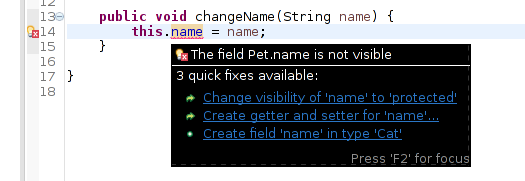
\includegraphics[scale=.8]{img/privatefieldnotvisible.png}
    \end{figure}
\end{frame}

\begin{frame}{Sichtbarkeitsmodifizierer in Java}
    \begin{figure}
        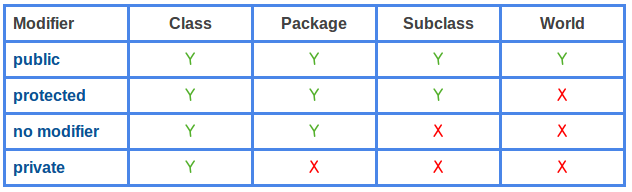
\includegraphics[scale=.4]{img/pppp.png}
    \end{figure}
\end{frame}


\section{Polymorphismus}

\begin{frame}{Polymorphismus}
    \begin{figure}
        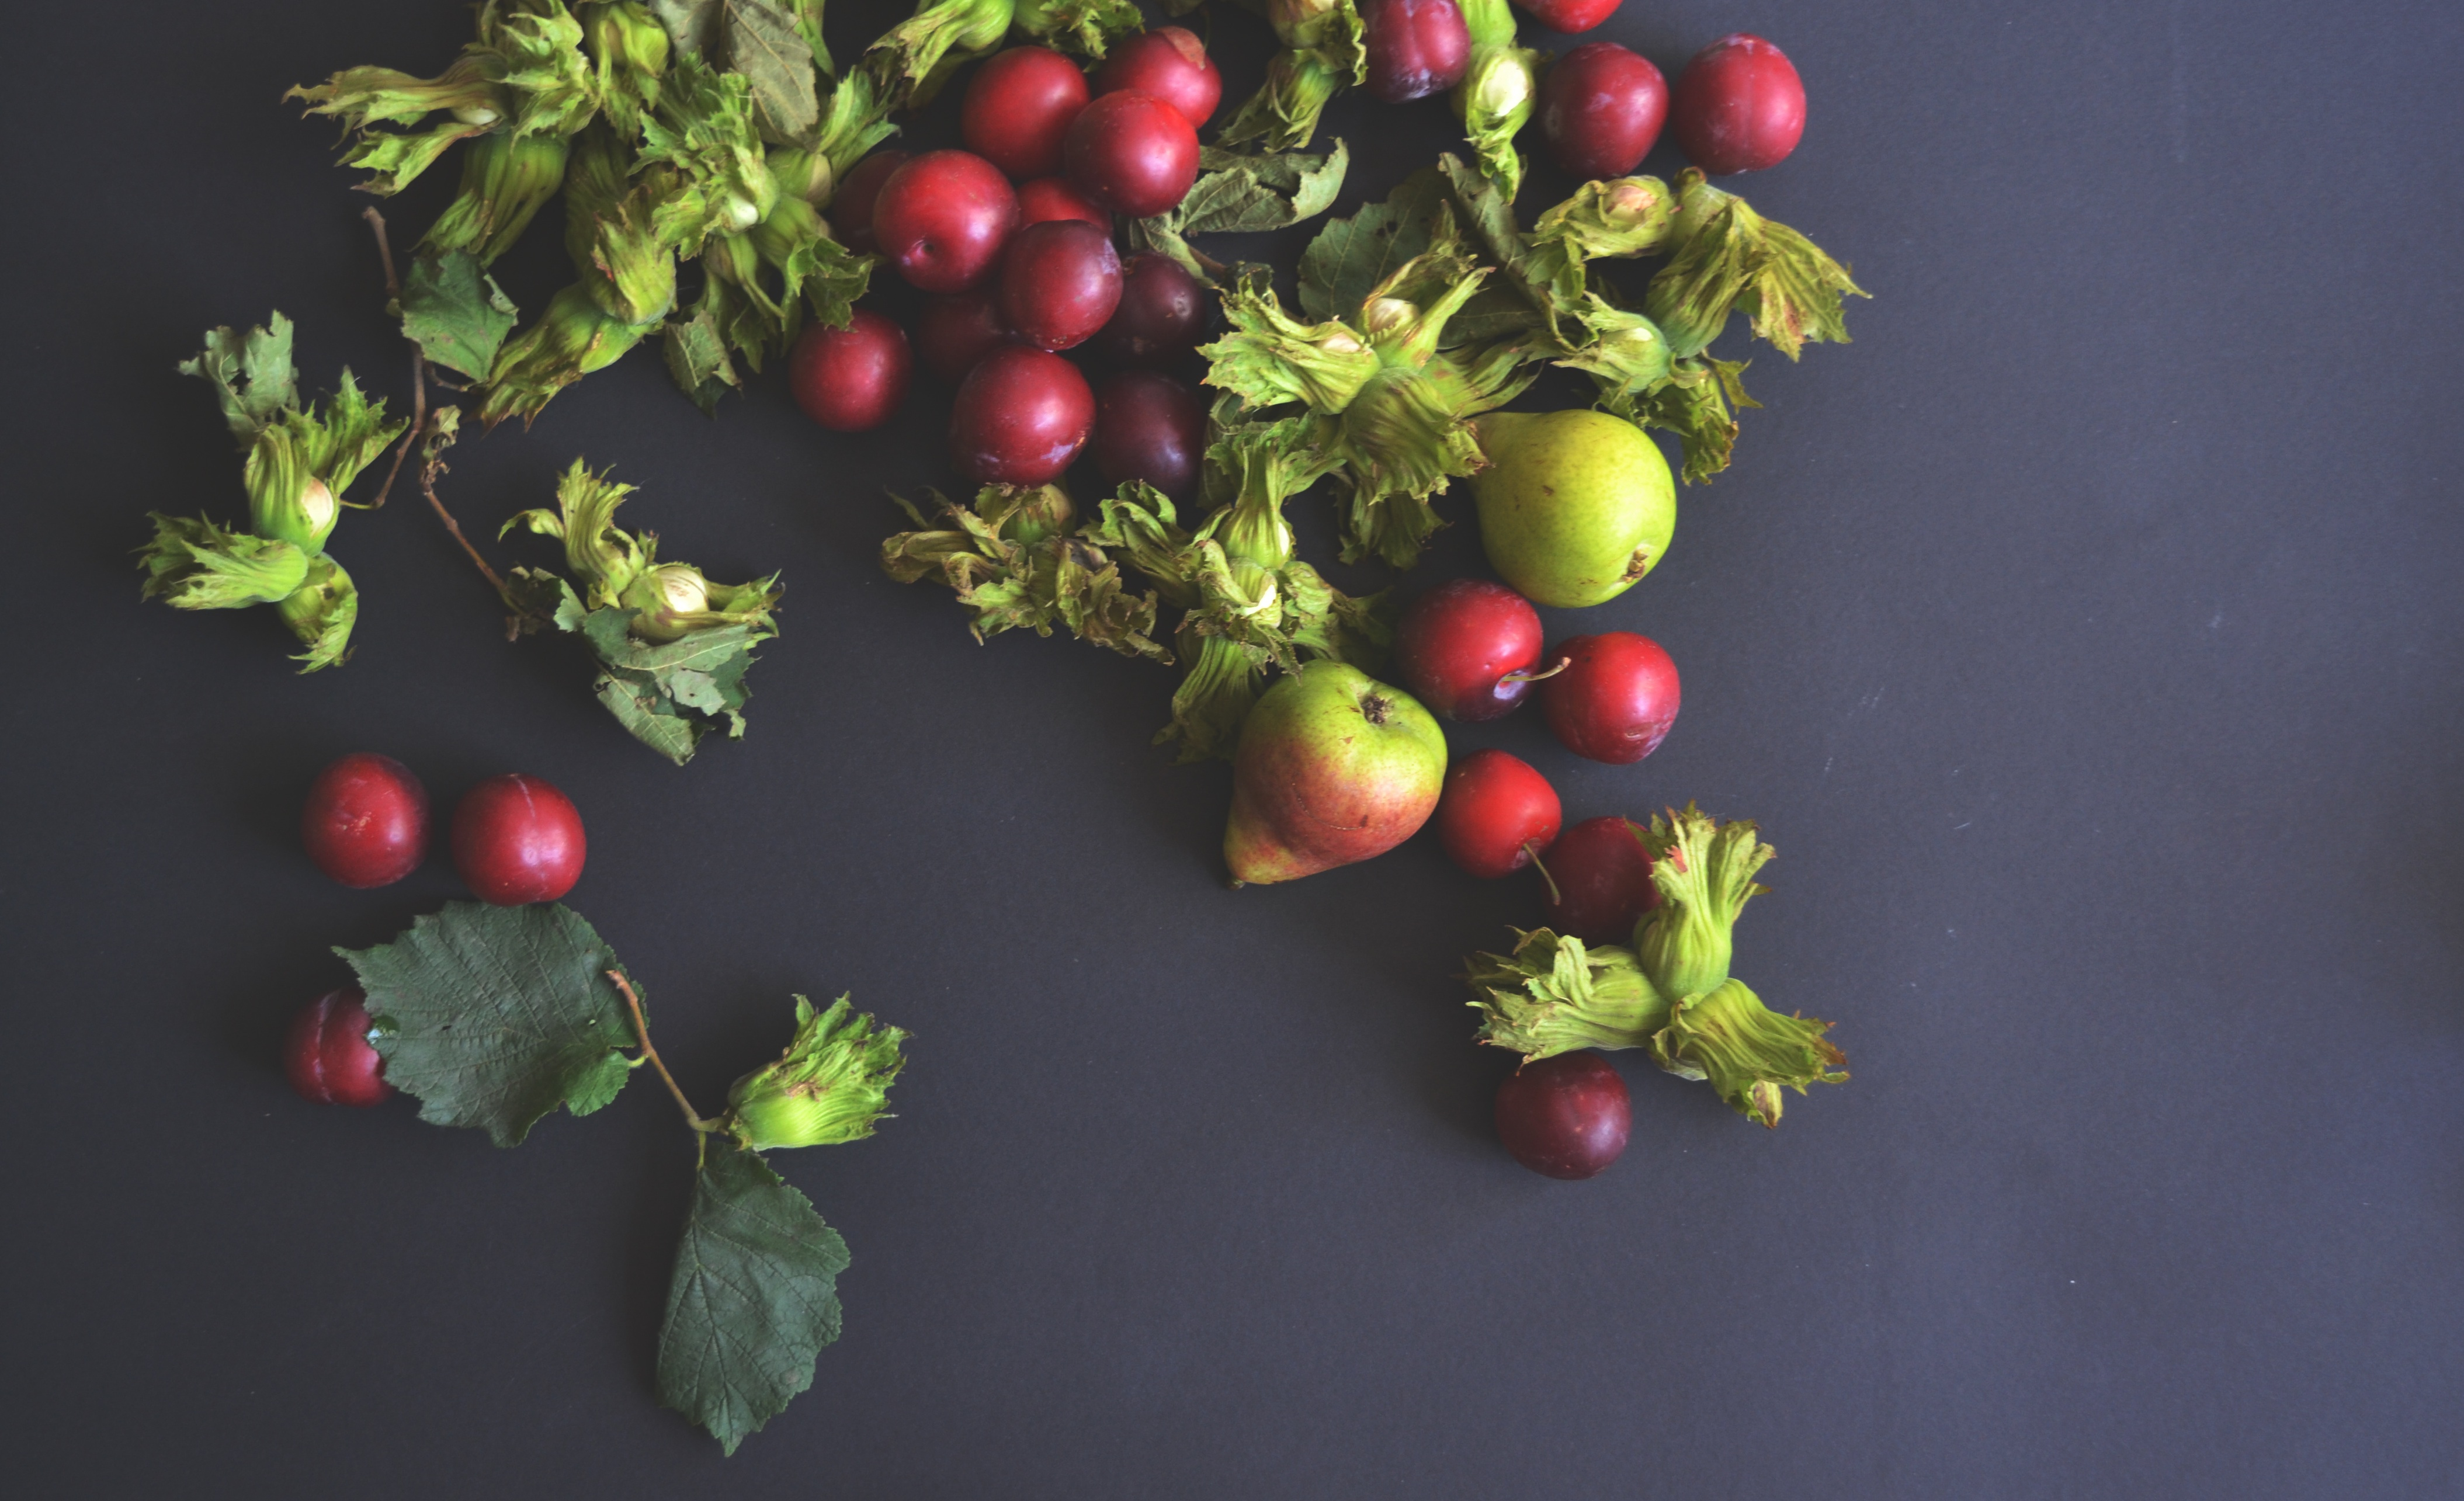
\includegraphics[scale=.075]{img/L18DEQZJQI.jpg}
    \end{figure}
\end{frame}

\begin{frame}{Polymorphismus}
    Was hat Polymorphismus mit Obst zutun ?
\end{frame}

\begin{frame}{Polymorphismus: Beispiel mit Obst}
    \begin{itemize}
        \item Sei \texttt{Fruit} eine Klasse
        \item \texttt{Mango}, \texttt{Ananas}, \texttt{Orange} seien Unterklassen von \texttt{Fruit}
        \pause
        \vspace{.3in}
        \item Alle Objekte vom Typ \texttt{Fruit} sollen eine Methode \texttt{consume()} haben
    \end{itemize}
        \pause
        \vspace{.3in}
        \textbf{Problem:} \texttt{consume()} kann nicht sinnvoll in \texttt{Fruit} implementiert werden !
\end{frame}

\begin{frame}{Polymorphismus: Beispiel mit Obst}

    \begin{itemize}
        \item Die Methode \texttt{consume()} muss in jeder Unterklasse (\texttt{Mango}, \texttt{Ananas}, \texttt{Orange}\dots) \textit{unterschiedlich} implementiert werden
        \item Unterklassen von \texttt{Fruit} können sich also beim Aufruf von \texttt{consume()} \textit{unterschiedlich} verhalten
    \end{itemize}

    \pause
    \vspace{.2in}

    Dieses Konzept bezeichnet man als \textbf{Polymorphismus}.
\end{frame}

\begin{frame}{Polymorphismus}
    Eine Methode ist \textbf{polymorph}, wenn sie in verschiedenen Klassen die gleiche Signatur hat,
    jedoch erneut implementiert ist.

\end{frame}

\begin{frame}[fragile]{Overriding:\\ Überschreiben von Methoden}
    \begin{exampleblock}{}
        \begin{lstlisting}[language=Java,basicstyle=\scriptsize]
public class Orange extends Fruit {

    @Override
    public void consume() {
        System.out.println("Peel first, then eat.");
    }

}
        \end{lstlisting}

    \end{exampleblock}

\end{frame}

\begin{frame}[fragile]{Overloading versus Overriding}
    \begin{columns}[c]
        \column{.5\textwidth}
        \begin{exampleblock}{Overloading}
            \begin{lstlisting}[language=Java,basicstyle=\scriptsize]
public class Color {

    public Color(
        int red, int green, int blue)
        { ... }

    public Color(String hex) { ... }

}
            \end{lstlisting}

        \end{exampleblock}

        \column{.5\textwidth}

        \begin{exampleblock}{Overriding}
            \begin{lstlisting}[language=Java,basicstyle=\scriptsize]
public class Fruit {

    public void consume() { ... }

}

public class Ananas extends Fruit {

    @Override
    public void consume() { ... }

}
            \end{lstlisting}

        \end{exampleblock}

    \end{columns}
\end{frame}


\subsection{Subtyping}

\begin{frame}{Subtyping}
    \begin{block}{}
        \begin{itemize}
            \item Es ist erlaubt, Objekte einer Unterklasse im Kontext der Oberklasse zu verwenden.
            \item \quotes{Jedes \texttt{A} ist auch ein \texttt{B}}
        \end{itemize}
    \end{block}

\end{frame}

\begin{frame}[fragile]{Subtyping}
    \begin{itemize}
        \item \quotes{Every \texttt{Orange} is a \texttt{Fruit}}
        \item Wenn ein Objekt vom Typ \texttt{Fruit} erwartet wird, dann ist \texttt{Orange} auch erlaubt
    \end{itemize}

    \begin{exampleblock}{}
        \begin{lstlisting}[language=Java]
Fruit f = new Orange();  // yes

Orange o = new Fruit();  // no
        \end{lstlisting}

    \end{exampleblock}
\end{frame}


\begin{frame}{Substitutionsprinzip}
    \begin{block}{}
        Das \textbf{Liskovsche Substitutionsprinzip} (LSP) besagt,
        dass ein Programm, das Objekte einer Basisklasse verwendet,
        auch mit Objekten der davon abgeleiteten Unterklasse korrekt funktionieren muss.
    \end{block}

\end{frame}

\begin{frame}{Substitutionsprinzip}
    \begin{itemize}
        \item Ein Programm, das mit Objekten vom Typ \texttt{Fruit} klarkommt, sollte ebenfalls mit Objekten vom Typ \texttt{Orange} funktionieren
        \item Eine \texttt{Orange} sollte also besser keine \quotes{bösen Überraschungen} mit sich bringen
        \item Ein \texttt{Orange}-Objekt sollte mindestens so viel können, wie ein \texttt{Fruit}-Objekt, oder mehr !
    \end{itemize}
\end{frame}

\begin{frame}{Subtyping vs. Substitutionsprinzip}
    \begin{alertblock}{Wichtig}
        \begin{itemize}
            \item \textbf{Subtyping} betrifft nur die Syntax (i.e., Java erlaubt es)
            \item \textbf{Substitutionsprinzip} einzuhalten ist Aufgabe des Programmierers
        \end{itemize}
    \end{alertblock}

\end{frame}

\subsection{Dynamische Bindung}

\begin{frame}{Dynamische Bindung}
    \begin{block}{}
        Man spricht von \textbf{dynamischer Bindung}, wenn ein Methodenaufruf \textbf{zur Laufzeit} anhand
        des tatsächlichen (dynamischen) Typs eines Objektes aufgelöst wird.
    \end{block}

\end{frame}


\begin{frame}[fragile]{Dynamische Bindung}
    \begin{exampleblock}{Fruit versus Orange}
        \begin{lstlisting}[language=Java,basicstyle=\scriptsize]
public class Fruit {

    public void consume() {
        System.out.println("Just eat it.");
    }

}

public class Orange extends Fruit {

    @Override
    public void consume() {
        System.out.println("Peel first, then eat.");
    }

}
        \end{lstlisting}

    \end{exampleblock}

\end{frame}

\begin{frame}[fragile]{Dynamische Bindung}
    \begin{exampleblock}{Was kommt raus ?}
        \begin{lstlisting}[language=Java]
Fruit first = new Fruit();
Fruit second = new Orange();

first.consume();
second.consume();
        \end{lstlisting}

    \end{exampleblock}

\end{frame}

\begin{frame}[fragile]{Dynamische Bindung}
    \begin{exampleblock}{Ausgabe}
        \begin{lstlisting}
Just eat it.
Peel first, then eat.
        \end{lstlisting}
    \end{exampleblock}

    \begin{itemize}
        \item Der statische Typ von \texttt{second} ist zwar \texttt{Fruit}, aber \textbf{zur Laufzeit} ist der \alert{dynamische Typ} \texttt{Orange} !
        \item Java entscheidet sich deshalb zur Laufzeit doch noch für den Code der \texttt{Orange}-Methode.
    \end{itemize}

\end{frame}



\begin{frame}[fragile]{super}
    Das Schlüsselwort \textbf{super} erlaubt den Zugriff auf Methoden der Oberklasse.

    \begin{exampleblock}{}
        \begin{lstlisting}[language=Java]
public class Dog extends Pet {

    public void sayName() {
        System.out.print("Wauwau ");
        super.sayName();
    }

}
        \end{lstlisting}

    \end{exampleblock}

\end{frame}

\begin{frame}[fragile]{super}
    Mit \textbf{super} kann man auch den \textbf{Konstruktor der Oberklasse} aufrufen.

    \begin{exampleblock}{}
        \begin{lstlisting}[language=Java]
public class Dog extends Pet {

    public Dog(String name) {
        super(name);
    }

}
        \end{lstlisting}

    \end{exampleblock}
    \vspace{.2in}
    Jetzt haben wir endlich den Konstruktor der \texttt{Pet}-Klasse übernommen !
\end{frame}

\subsection{Abstrakte Klassen}

\begin{frame}{Abstrakte Klassen}
    Mit dem Schlüsselwort \textbf{abstract} kann man eine Klasse als \quotes{reine Oberklasse} deklarieren.

    \begin{itemize}
        \item Abstrakte Klassen können nicht direkt instanziiert werden
        \item Keine oder unvollständige Implementierung
        \item Methoden können ebenfalls als \textbf{abstract} deklariert werden, wenn sie in der abstrakten Klasse (noch) nicht implementiert werden
    \end{itemize}
\end{frame}

\begin{frame}[fragile]{Abstrakte Klassen}
    \begin{exampleblock}{}
        \begin{lstlisting}[language=Java,basicstyle=\scriptsize]
public abstract class Fruit {
    public abstract void consume();
}

public class Orange extends Fruit {

    @Override
    public void consume() {
        System.out.println("Peel first, then eat.");
    }

}
        \end{lstlisting}

    \end{exampleblock}

    \begin{itemize}
        \item \texttt{abstract class Fruit} : die Klasse \texttt{Fruit} kann nicht direkt instanziiert werden
        \item \texttt{abstract void consume()} : die Methode \texttt{consume()} wird nicht hier implementiert
    \end{itemize}

\end{frame}

\begin{frame}{Abstrakte Klassen}
    \begin{block}{}
        \textbf{Korollar:}\\
        Eine Klasse mit abstrakten Methoden muss abstrakt sein.
    \end{block}

\end{frame}



\begin{frame}{final}
    \begin{itemize}
        \item Mit dem Schlüsselwort \textbf{final} kann man eine Klasse als \quotes{nicht mehr erweiterbar} deklarieren
        \item Finale Klassen können also nicht mehr als Oberklasse verwendet werden
        \item Verhalten wird fixiert
    \end{itemize}
\end{frame}

\begin{frame}{Interfaces}
    \textbf{Interfaces} stellen Schnittstellen dar.
    \begin{itemize}
        \item Ein Interface ist eine Sammlung von Methodensignaturen \textit{ohne} Implementierung
        \item Eine Klasse kann ein \textbf{Interface} implementieren
        \item Die implementierende Klasse muss dann \textbf{jede Methode} des Interfaces implementieren
        \item Eine Klasse kann auch \textbf{mehrere Interfaces} gleichzeitig implementieren
    \end{itemize}
\end{frame}

\begin{frame}[fragile]{Interfaces}
    \begin{exampleblock}{}
        \begin{lstlisting}[language=Java,basicstyle=\scriptsize]
public interface Eatable {

    public void consume();

}
        \end{lstlisting}

    \end{exampleblock}

    \begin{exampleblock}{}
        \begin{lstlisting}[language=Java,basicstyle=\scriptsize]
public class Orange implements Eatable {

    @Override
    public void consume() {
        System.out.println("Peel first, then eat.");
    }

}
        \end{lstlisting}

    \end{exampleblock}

\end{frame}

\begin{frame}[fragile]{Interfaces}

    Das geht auch\dots

    \begin{exampleblock}{}
        \begin{lstlisting}[language=Java,basicstyle=\scriptsize]
public abstract class Fruit implements Eatable {

    @Override
    public abstract void consume();

}
        \end{lstlisting}

    \end{exampleblock}
\end{frame}


\begin{frame}[fragile]{instanceof-Operator}
    Mit \textbf{instanceof} kann geprüft werden, ob ein gegebenes Objekt von einem bestimmten Typ ist.

    \begin{exampleblock}{}
        \begin{lstlisting}[language=Java,basicstyle=\scriptsize]
Fruit fruit;
// ...

if (fruit instanceof Orange) {
    System.out.println("This is an Orange.");
} else {
    System.out.println("This is a random Fruit.");
}
        \end{lstlisting}

    \end{exampleblock}

    \pause

    \alert{\textbf{instanceof} sollte sehr sparsam verwendet werden !}

\end{frame}

\begin{frame}[fragile]{Typecast}
    \begin{lstlisting}
(Type) variable
    \end{lstlisting}

    \vspace{.2in}
    \begin{itemize}
        \item Up-Cast
            \begin{itemize}
                \item ist immer erlaubt, da \textbf{is-a} Beziehung gilt
                \item wird bei Zuweisungen und Methodenaufrufen implizit ausgeführt
            \end{itemize}
        \item Down-Cast
        \begin{itemize}
            \item kann zu Laufzeitfehler führen !
            \item ist immer explizit
            \item sollte vorher mit \textbf{instanceof} geprüft werden
        \end{itemize}
    \end{itemize}
\end{frame}

\section{Debugging}

\begin{frame}{Debugging}
    \begin{figure}
        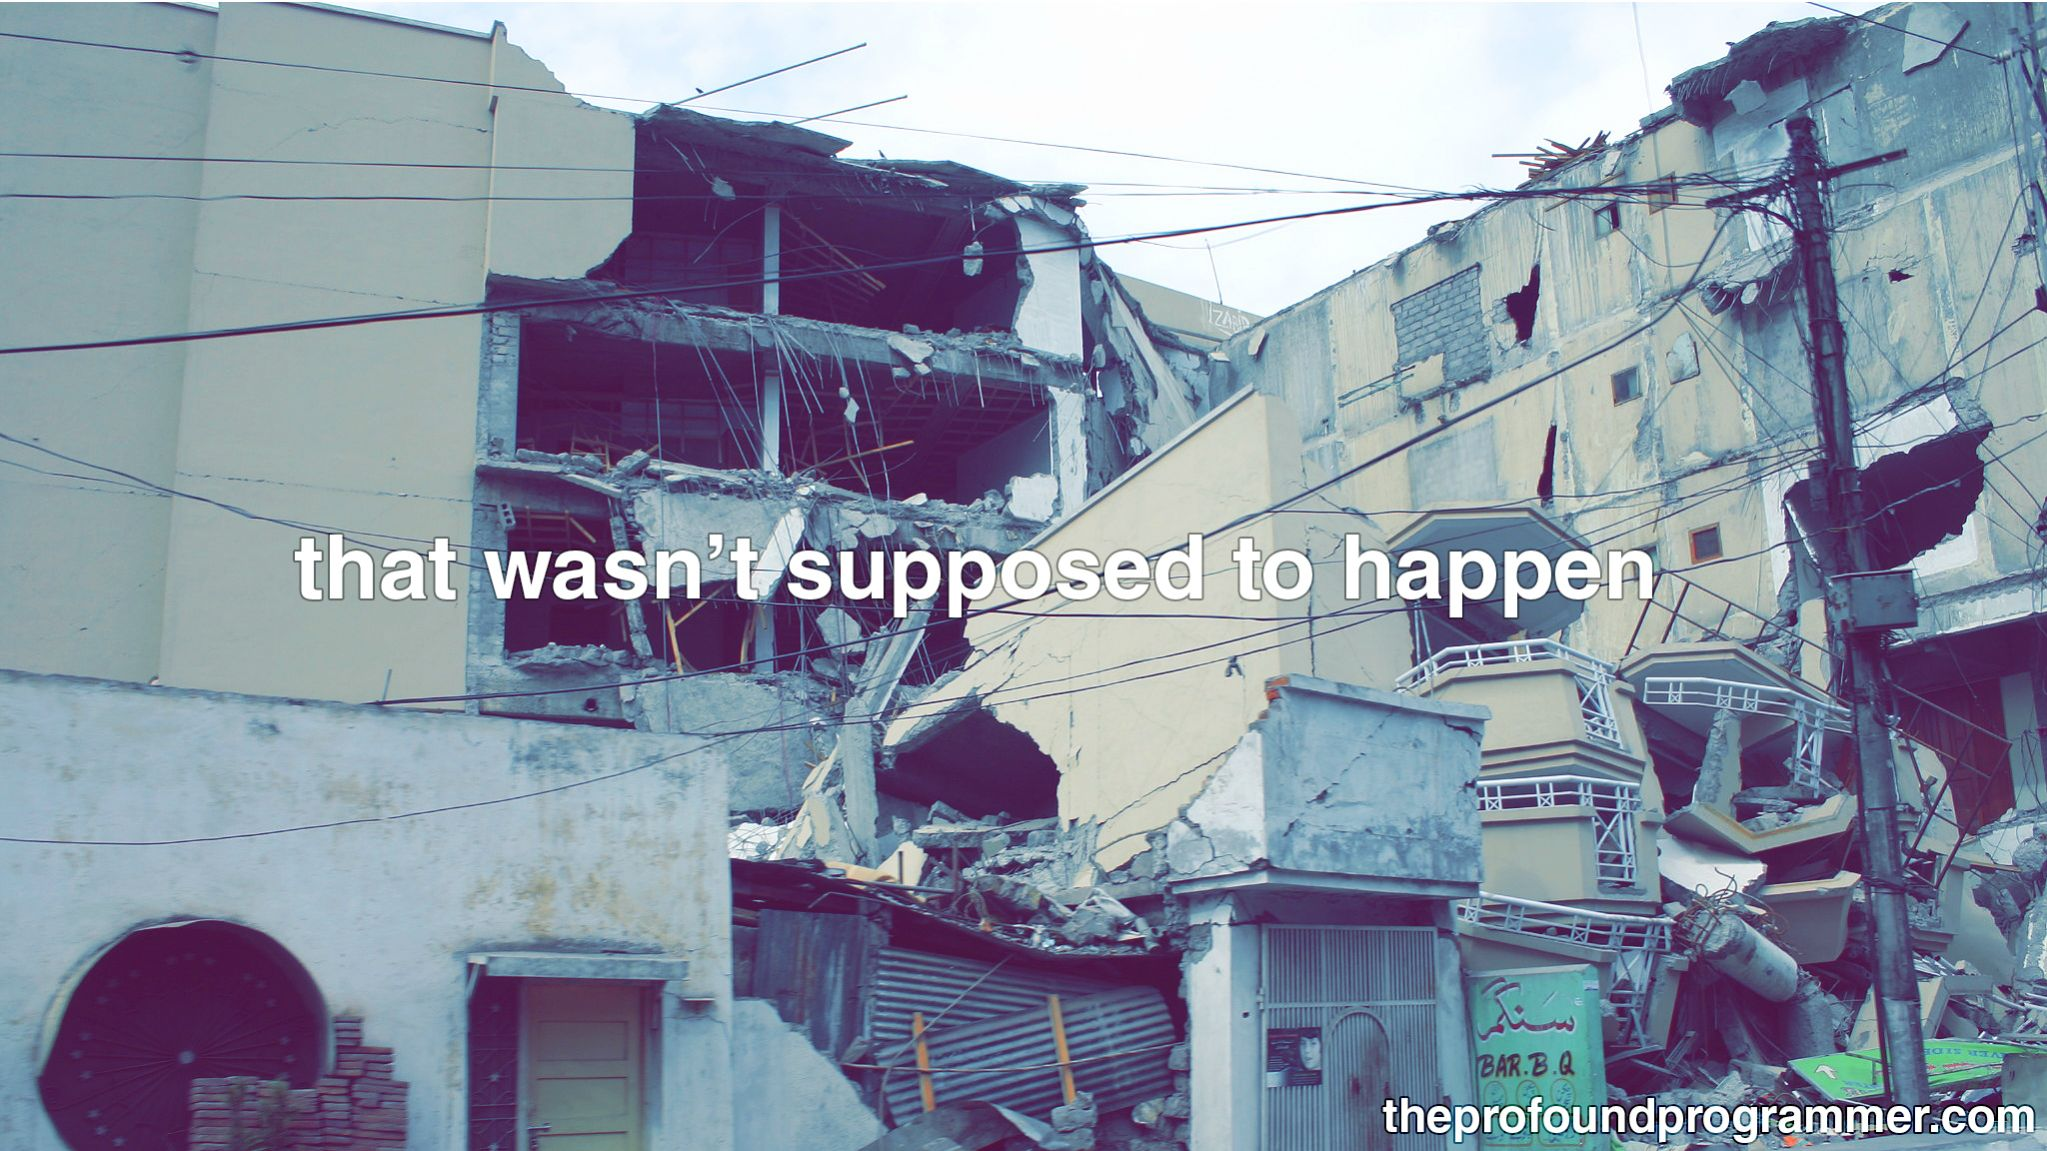
\includegraphics[scale=.15]{img/NG8XW8J8GT.jpg}
    \end{figure}
\end{frame}

\begin{frame}{Debugging}
    \textbf{Debugging}: Finden und Entfernen von Fehlern (Bugs) in einem Programm
\end{frame}

\begin{frame}{Debugging}
    Praktische Tipps:
    \begin{itemize}
        \item Code erneut durchlesen
        \item Verschiedene Eingaben testen und genau auf Resultat achten
        \item Inhalte an verschiedenen Stellen im Programm ausgeben lassen
        \item An geeigneten Stellen feste Werte reinschreiben und schauen was dann passiert
        \item Debugger verwenden
        \item \dots
    \end{itemize}
\end{frame}

\appendix
\beginbackup

\begin{frame}{Programmieren-Wiki}
    Es gibt eine \textbf{Programmieren-Wiki} im ILIAS mit u.a. folgenden Inhalten:

    \begin{itemize}
        \item Debugging
        \item Eclipse IDE
        \item Checkstyle
        \item Programmierstil
        \item Javadoc
        \item \dots
    \end{itemize}
\end{frame}


\begin{frame}{Fragen ?}
    \begin{figure}
        
\includegraphics[scale=.6]{img/additionalquestions.jpg}
    \end{figure}
\end{frame}

\begin{frame}{Bis nächste Woche !}
    \begin{figure}
        
\includegraphics[scale=.6]{img/dilbert-software-demo.jpg}
    \end{figure}
\end{frame}

\backupend

\end{document}
